\documentclass{beamer}
\usetheme{Boadilla}

\usepackage{amsmath}
\usepackage{amsfonts}
\usepackage{hyperref}



\title{Generative alternatives}
\author{Skorik Sergey}
\institute{MIPT, 2023}


\begin{document}

\begin{frame}
    \titlepage
\end{frame}

\begin{frame}
    \tableofcontents
\end{frame}

\section{Backgrounds}
\begin{frame}{Backgrounds}
    \begin{block}{State-space representation}
        The most general state-space representation of a linear system with $p$ inputs, $q$ outputs and $n$ state variables is written in the following form:
        \begin{equation}\label{SSR}
            \begin{cases}
                \Dot{x}(t) = \mathbf{A}(t)x(t) + \mathbf{B}(t)u(t) \\
                y(t) = \mathbf{C}(t)x(t) + \mathbf{D}(t)u(t)
            \end{cases}
        \end{equation}
    \end{block}
    \begin{figure}
        \centering
        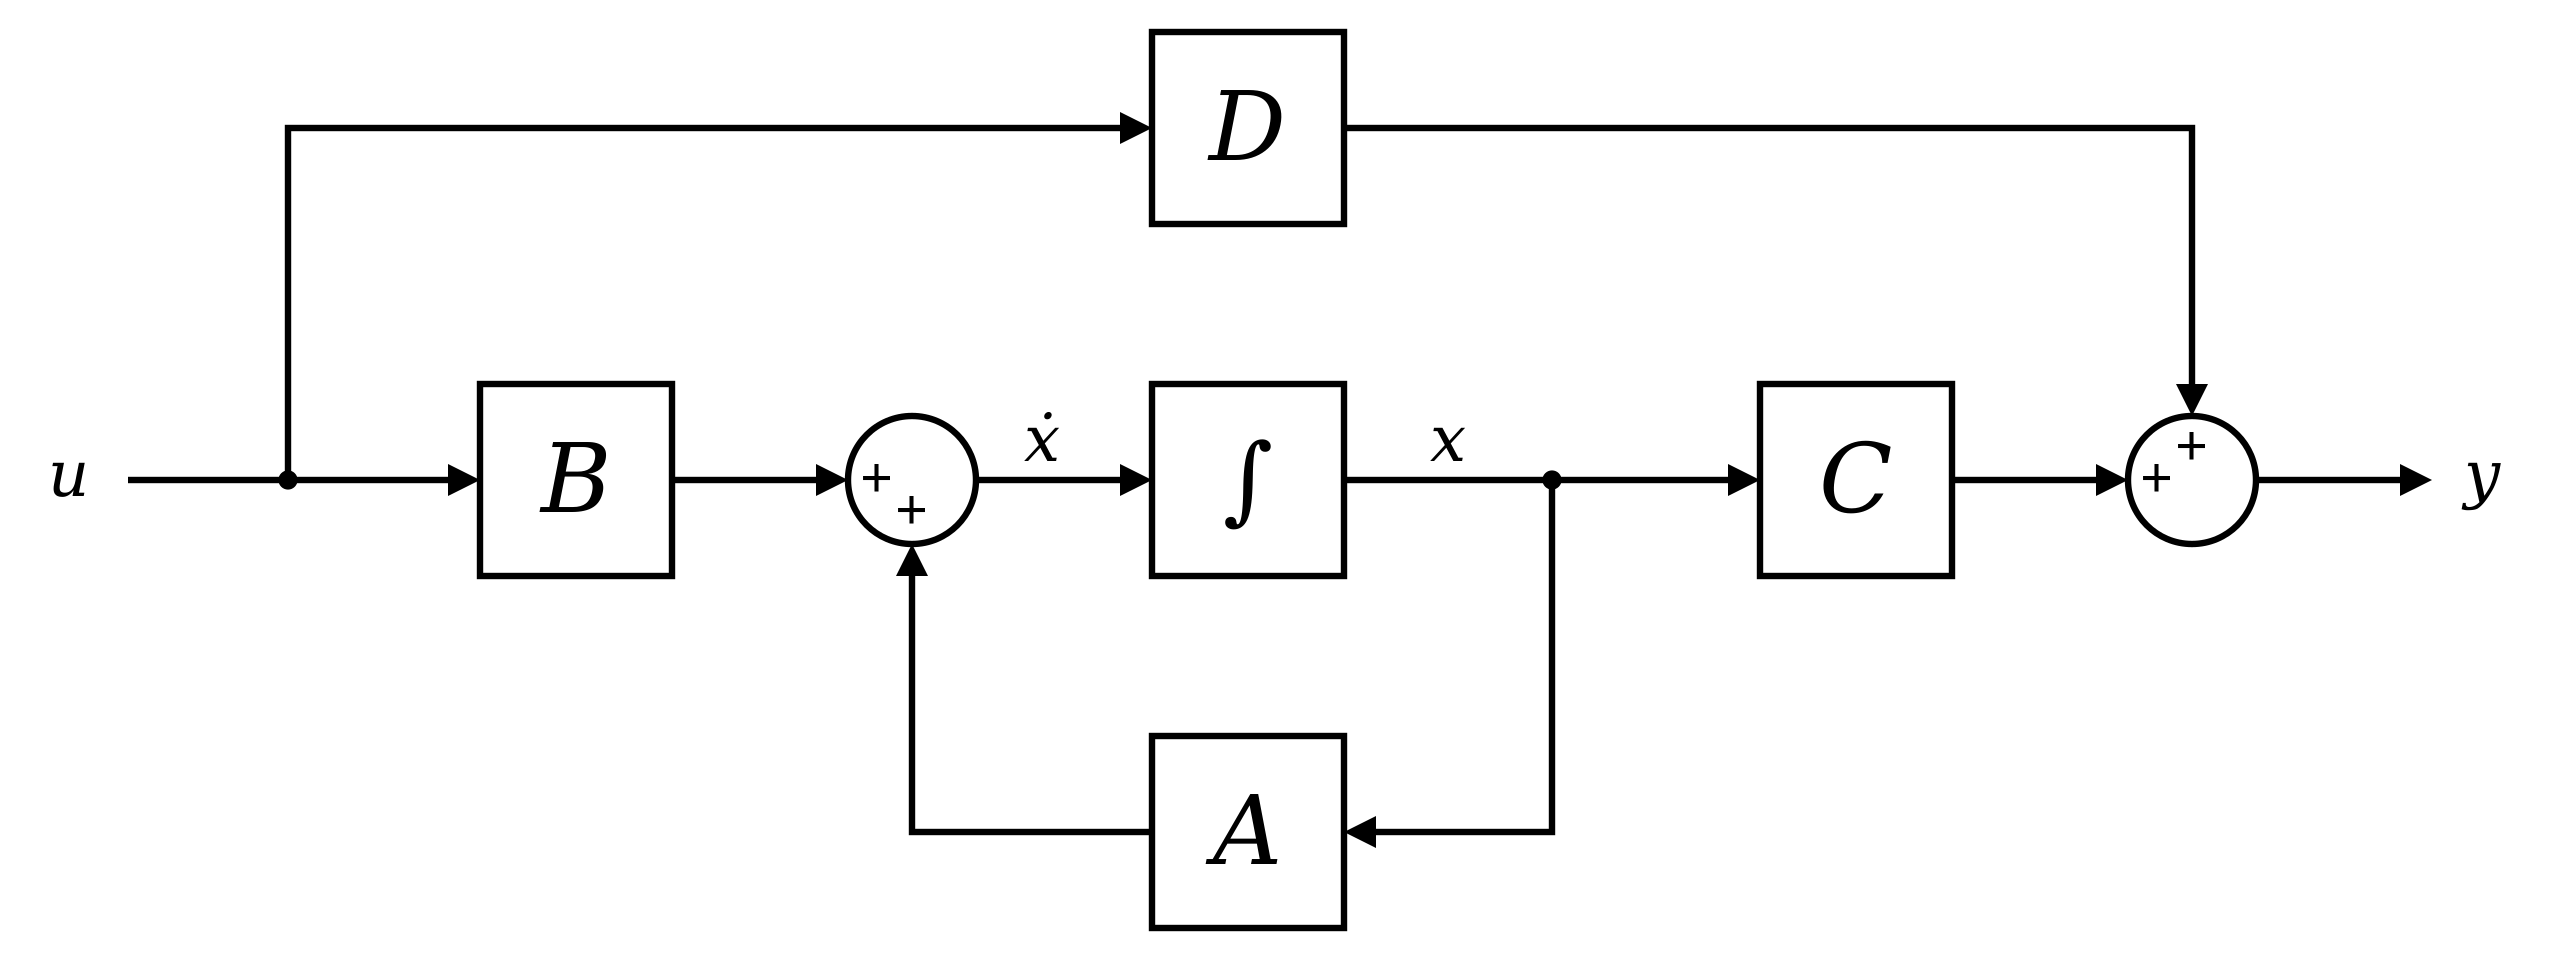
\includegraphics[scale=0.1]{space_state_repr.png}
    \end{figure}
\end{frame}

\begin{frame}{Backgrounds}
    \begin{block}{State-Space representation}
        State-Space representation is a mathematical model of a physical system. For example, for mass spring damper system (https://cookierobotics.com/008/) the following equations describes them:
        \begin{equation}\label{MSDS}
            \begin{cases}
            \begin{bmatrix}
                \Dot{x}_1(t) \\
                \Dot{x}_2(t)
            \end{bmatrix} = \begin{bmatrix}
                0 & 1 \\
                - \frac{k}{m} & - \frac{b}{m}
            \end{bmatrix} \cdot \begin{bmatrix}
                x_1(t) \\
                x_2(t)
            \end{bmatrix} + \begin{bmatrix}
                0 \\
                \frac{1}{m}
            \end{bmatrix} \cdot \begin{bmatrix}
                u(t)
            \end{bmatrix} \\
            
            \begin{bmatrix}
                y(t)
            \end{bmatrix}  = \begin{bmatrix}
                1 & 0
            \end{bmatrix} \cdot \begin{bmatrix}
                x_1(t) \\
                x_2(t)
            \end{bmatrix}
            \end{cases}
        \end{equation}
        eal-world dynamics might not be fully known or may be subject to uncertainty. In such cases, $A$ is used to capture the probabilistic or stochastic nature of the state dynamics. Instead of being a fixed matrix, $A$ is modeled as a distribution over possible state transitions $A \sim \mathcal{N}(\mu, \Sigma)$.
    \end{block}
\end{frame}
\section{HiPPO}

\begin{frame}{HiPPO Framework}
    \begin{figure}
        \centering
        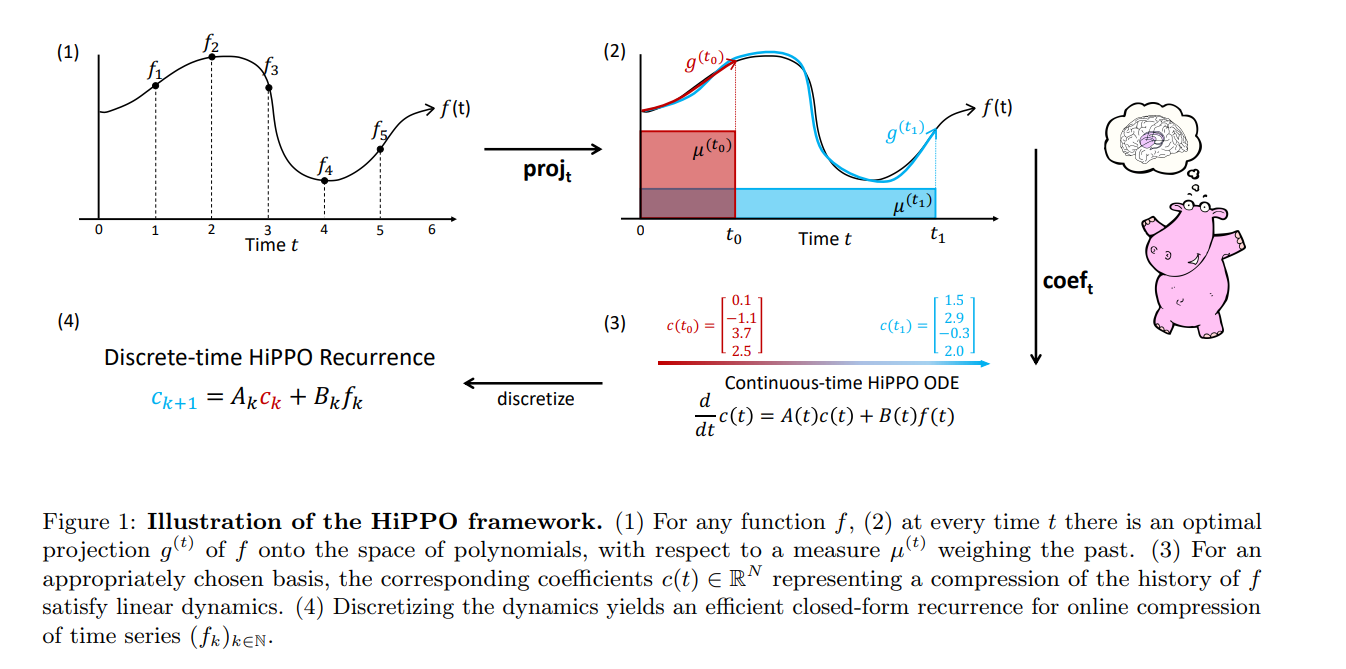
\includegraphics[scale=0.25]{hippo.png}
    \end{figure}
\end{frame}

\begin{frame}{HiPPO Framework}
    \begin{block}{Connection between SSR and HiPPO}
        The composition $coef \circ proj$ is called hippo, which is an operator mapping a function $f$ to the optimal projection coefficients $c$, i.e. $(hippo(f))(t) = coef_t(proj_t(f))$. The coefficient function $c(t) = coef_t(proj_t(f))$ has the form of an ODE satisfying $\dot{c}(t) = A(t)c(t) + B(t)f(t)$
    \end{block}
    
\end{frame}


\begin{frame}{SSM setup}
    \begin{block}{SSM setup}
        The state space model maps a 1-D input signal $u(t)$ to an N-D latent state $x(t)$ before projecting to a 1-D output signal $y(t)$
        \begin{equation}\label{SSM_cont}
            \begin{cases}
                \Dot{x}(t) = \mathbf{A}x(t) + \mathbf{B}u(t) \\
                y(t) = \mathbf{C}x(t)
            \end{cases}
        \end{equation}
        The discrete SSM is
        \begin{equation}\label{SSM_disc}
            \begin{cases}
                x_k = \bar{\mathbf{A}}x_{k-1} + \bar{\mathbf{B}}u_k, \quad  \bar{\mathbf{A}} = (\mathbf{I} - \Delta / 2\cdot \mathbf{A})^{-1}(\mathbf{I} + \Delta / 2\cdot \mathbf{A}) \\
                y_k = \bar{\mathbf{C}}x_{k}, \quad \bar{\mathbf{B}} = (\mathbf{I} - \Delta / 2\cdot \mathbf{A})^{-1}\Delta\mathbf{B}, \quad \bar{\mathbf{C}} = \mathbf{C}
            \end{cases}
        \end{equation}
        The fundamental bottleneck in computing the discrete-time SSM \eqref{SSM_disc} is that it involves repeated matrix multiplication by $\bar{\mathbf{A}}$. For example, naively as in the LSSL involves L successive multiplications
        by $\bar{\mathbf{A}}$ requiring $\mathcal{O}(N^2\cdot L)$ operations and $\mathcal{O}(NL)$ space. 
    \end{block}
\end{frame}

\begin{frame}{HiPPO}
    \begin{block}{HiPPO}
        HiPPO specifies a class of certain matrices $\mathbf{A} \in \mathbb{R}^{N\times N}$ that when incorporated into \eqref{SSM_cont}, allows the state $x(t)$ to memorize the history of the input $u(t)$.
        \begin{equation}\label{HiPPO}
            (\textbf{HiPPO Matrix}) \quad \mathbf{A}_{nk} = - \begin{cases}
                (2n+1)^{1/2}(2k+1)^{1/2} & \text{if}\, n > k \\
                n + 1 & \text{if}\, n = k \\
                0 & \text{if}\, n < k \\
            \end{cases}
        \end{equation}
        The ideal scenario is when the matrix $\mathbf{A}$ is diagonalizable by a perfectly conditioned (i.e., unitary) matrix. By the Spectral Theorem of linear algebra, this is exactly the class \textbf{normal matrices}. In particular, it does not contain the HiPPO matrix.
    \end{block}
\end{frame}

\section{S4}

\begin{frame}{S4}
    \begin{figure}
        \centering
        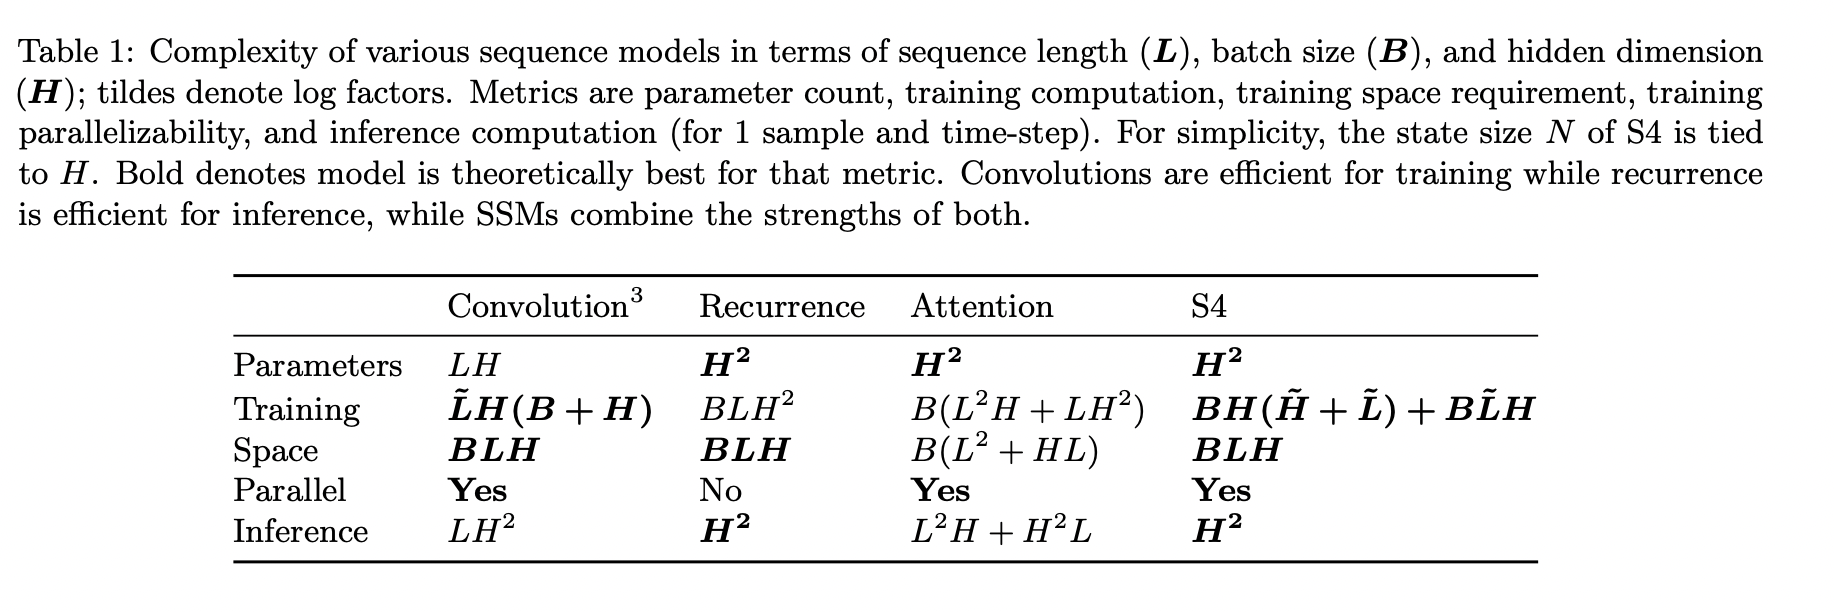
\includegraphics[scale=0.35]{comparsion.png}
    \end{figure}
\end{frame}

\section{Kalman Filter}

\begin{frame}{Kalman Filter}
    \begin{figure}
        \centering
        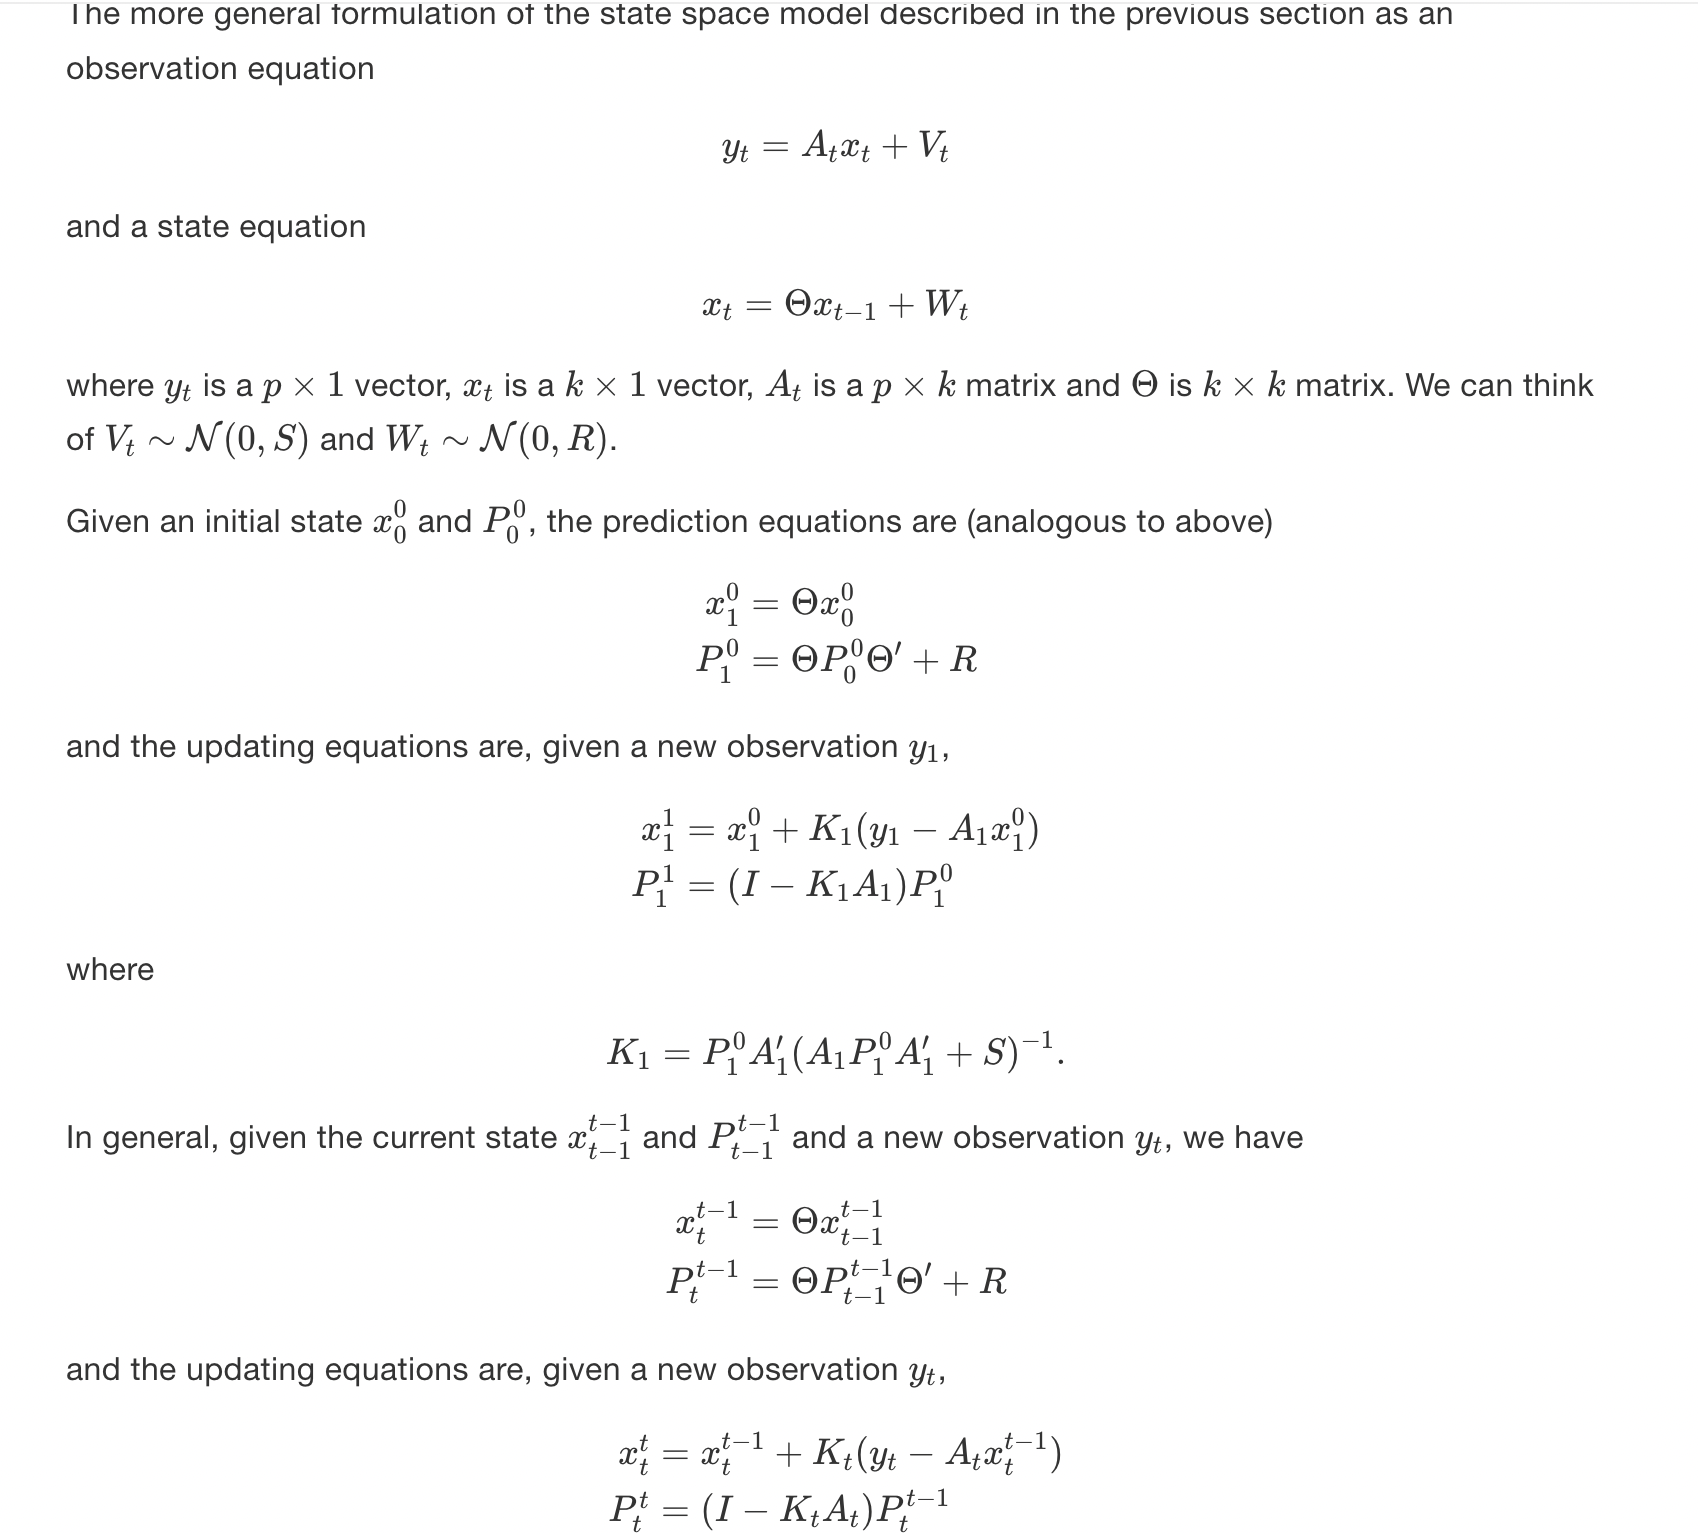
\includegraphics[scale=0.35]{Kalman.png}
    \end{figure}
\end{frame}
\end{document}
